\InputIfFileExists{../data/global.src}\relax\relax

\iffull
\title{Sichtbar ungültige Seiteneffekte!}
\subtitle{Tutorium sechs}
\date{KW 24}
\addbibresource{references.bib}
\fi
\SetTutoriumNumber{6}

\iffull\begin{document}
\titleframe

\TopicOverview{7}
\fi
\iffull{\SummaryFrame
\def\sub#1#2{\node[font=\footnotesize\sffamily,scale=.715,align=center,gray,below=-2.65mm] at(#1.south) {\strut#2\strut};}
\setbeamerfont{description item}{series=\mdseries,shape=\itshape}
\begin{frame}[c]{Algorithmen}
\begin{itemize}[<+(1)->]
   \itemsep14pt
   \item Totale Korrektheit \begin{description}[Partielle Korrektheit: ]
      \item[Terminiertheit:] \strut\onslide<+(1)->{Endliche Schritte für jede Eingabe}
      \item[Partielle Korrektheit:] \strut\onslide<+(1)->{Wenn terminiert, dann korrekt}
   \end{description}
   \item Weitere Eigenschaften \begin{description}[Determiniertheit: ]
      \item[Determiniertheit:] \strut\onslide<+(1)->{Gleiche Eingabe~\(\to\) Gleiche Ausgabe}
      \item[Determinismus:] \strut\onslide<+(1)->{Gleiche Eingabe~\(\to\) Gleiche Zustandsfolge}
   \end{description}
\end{itemize}\vfill
\centerline{%
\begin{tikzpicture}
    \onslide<+(1)->{\node (0) at(0,0) {\strut Spezifikation};
    \sub0{Begriffe mit\\Problemrelevanz}}
    \foreach[count=\i,remember =\i as \li (initially 0)] \a/\t in {Abstraktion/{Gegeben \& Gesucht},{\makebox[14mm]{\only<17->{\sbseries}Entwurf}}/{Algorithmus},Verifikation/{Termination \&\\partielle Korrektheit},Aufwandsanalyse/{Laufzeitverhalten}} {
        \onslide<+(1)->{\node[right=.5mm] (k\i) at(\li.east) {\strut\faAngleRight};
        \node[right=.5mm] (\i) at (k\i.east) {\strut\a};
        \sub\i{\t}}
    }
\end{tikzpicture}}
\end{frame}

\def\mto{\ensuremath{\to}}
\def\dt#1{{\textcolor{paletteA!58!white}{\sbseries\strut#1}}}
\begin{frame}[c]{Konstrukte}
\begin{itemize}[<+(1)->]
   \itemsep18pt
   \item \textit{Implizit}:\quad\pause \dt{byte}~\mto~\dt{short}~\mto~\dt{int}~\mto~\dt{long}~\mto~\dt{float}~\mto~\dt{double}\\
   Zahlen von klein zu groß, sowie: \dt{char}~\mto~\dt{int}
   \item \textit{Präzedenzregeln}:\pause\\
   Post vor Prä, sonst wie Arithmetik \& Logik
   \item \textit{Default-Werte}:\quad\pause Zahlen und Zeichen \bjava{0}, Boolean \bjava{false}, Rest \bjava{null}\pause\\
   Nur bei: Arrays, Instanz- und Klassenvariablen (\link{https://docs.oracle.com/javase/specs/jls/se17/html/jls-4.html\#jls-4.12.5}{JLS17~4.12.5})
   \item \textit{Überschatten}:\pause\\
   Lokaler Bezeichner überdeckt Gültigkeit des globalen
\end{itemize}
\end{frame}

\def\mto{\ensuremath{\to}}
\begin{frame}[c]{Arrays \& Iteration}
\begin{itemize}[<+(1)->]
   \itemsep18pt
   \item Arrays sind komplexe Datentypen
   \item Mehrdimensionale Arrays sind eindimensionale Arrays von eindimensionalen Arrays von\ldots
   \item Die drei Schleifenarten sind gleich mächtig \begin{itemize}
      \item Maximum bekannt: \bjava{for}
      \item Mindestens ein mal: \bjava{do}-\bjava{while}
      \item Sonst: \bjava{while}
   \end{itemize}
\end{itemize}
\end{frame}

\begin{frame}[c]{Unterprogramme}
\begin{itemize}[<+(1)->]
   \itemsep18pt
   \item \textit{Überladung:}\quad\pause Gleicher Name, andere Signatur \begin{itemize}
      \item \textit{Signatur:} \pause Name \& Parametertypliste
      \item Müssen zudem in selber Klasse sein (später: Vererbung)
   \end{itemize}
   \item Beim Aufruf macht Java call-by-value: \begin{itemize}
      \item Alle Parameter werden kopiert (Stack)
   \end{itemize}
   \item \bjava{void} gibt als Keyword an, dass die Methode keinen Rückgabetyp hat
\end{itemize}
\end{frame}

\begin{frame}[c]{Objektorientierte Progammierung}
\begin{itemize}[<+(1)->]
   \itemsep15pt
   \item Eine Klasse definiert die Blaupause für Objekte \begin{itemize}
      \item Attribute definieren den Zustand
      \item Methoden definieren den Verhalten
      \item Statische Elemente sind nicht Teil der Blaupause \info{sie gehören der Klasse!}
   \end{itemize}
   \item Der Konstruktor baut den initialen Zustand \begin{itemize}
      \item \textit{Instanziierung}: \pause Erzeugen eines neuen Objektes
      \item Wenn keiner: \pause erzeugt Java den leeren Standardkonstruktor
      \item \bjava{this} erlaubt Aufruf von überladenen Konstruktoren
   \end{itemize}
   \item Klassen, Methoden,~\ldots:\quad \textit{Sichtbarkeit} (\bjava{public},~\ldots)
   \item \textit{Gültigkeit}sbereich:\quad Wo die Variablen \say{deklariert sind} (Überschatten,~\ldots)
\end{itemize}
\end{frame}
}\fi

% TODO: make sectionlink auto triggerat start of section
\SetNextSectionText[.75\linewidth]{Ich glaub es bedarf weiterer Animationen.\smallskip\\ --- Break-Down-Flo}
\section{Präsenzaufgabe}
{\taskenum
\begin{frame}[fragile,c]{Präsenzaufgabe}
\begin{aufgabe}{Meine Kleine, du hast Palindrom!}
    \onslide<2->{In dieser Aufgabe sollen Sie eine rekursive Methode implementieren, die überprüfen soll, ob es sich bei dem als Parameter übergebenen String um ein Palindrom handelt. Ein Palindrom ist ein Wort, das vorwärts und rückwärts gelesen identisch ist.} \onslide<3->{Die Überprüfung soll nicht case-sensitive sein, d.h. das Wort \say{Kajak} soll zum Beispiel ein gültiges Palindrom sein.}

    \onslide<4->{Beantworten Sie zudem folgende Fragen bezüglich Ihrer Implementierung:}
    \begin{enumerate}
        \item<5-> Ist Ihre Implementierung ein linear-rekursiver Algorithmus? Warum?
        \item<6-> Ist Ihre Implementierung ein end- oder kopf-rekursiver Algorithmus? Warum?
    \end{enumerate}
\end{aufgabe}
\end{frame}
}

\begin{frame}[c,fragile]{Eine erste Idee}
    \onslide<2->{\only<3->{\color{gray}}In dieser Aufgabe sollen Sie eine {\color{black}rekursive Methode} implementieren, die überprüfen soll, ob es sich bei dem als {\color{black}Parameter übergebenen String} um ein {\color{black}Palindrom} handelt. Ein Palindrom ist ein Wort, das vorwärts und rückwärts gelesen identisch ist. Die Überprüfung soll {\color{black}nicht case-sensitive} sein, d.h. das Wort \say{Kajak} soll zum Beispiel ein gültiges Palindrom sein.}\bigskip

    \onslide<4->{\color{black}Idee:}
    \footnotesize\begin{itemize}
        \item<5-> Prüfe für \(i = 0\) bis \(i = \floor{\sfrac{\text{\bjava{s.length}}}{2}}\), ob \say{\bjava{s[i] == s[s.length - i - 1]}}.
        \item<6-> \bjava{String::toLowerCase()} entweder für jeden Vergleich oder einmal per Hilfsmethode.
        \item<7-> Noch einfacher: Anstelle \bjava{i} zu inkrementieren, löschen wir das erste und letzte Zeichen nach dem Vergleich (via \bjava{String::substring(int, int)}---das Ende ist exklusiv)!
    \end{itemize}
\end{frame}

\begin{frame}[fragile]{Von Palindromen}
\SetupLstHl\lstfs{10}%
\begin{plainjava}
!*\CodeFileMarkerAttach<2->{Palindrome.java}*!
!*\onslide<3->*!public static boolean isPalindrome(String s) { !*\Snode{@helper}*!
!*\onslide<4->*!    return isPalindromeRecursive(s.toLowerCase());
!*\onslide<3->*!}


!*\onslide<6->*!private static boolean isPalindromeRecursive(String s) {
!*\onslide<7->*!    if(s.length() < 2) !*\Snode{@1}*!
!*\onslide<8->*!        return true;
!*\onslide<10->*!    else if(s.charAt(0) != s.charAt(s.length() - 1)) !*\Snode{@2}*!
!*\onslide<10->*!        return false;
!*\onslide<7->*!    else !*\Snode{@3}*!
!*\onslide<9->*!        return isPalindromeRecursive(s.substring(1, s.length() - 1));
!*\onslide<6->*!}!*\onslide<1->*!
\end{plainjava}
\begin{tikzpicture}[@O]
    \onslide<5->{\node[T,yshift=.33mm,right] at(@helper) {die \say{Hilfsmethode}};}

    \onslide<7->{\node[T,yshift=.33mm,right] at(@1) {Basisfall: weniger als zwei Zeichen};}
    \onslide<9->{\node[T,yshift=.33mm,right] at(@2) {Basisfall: kein Palindrom!};}
    \onslide<7->{\node[T,yshift=.33mm,right] at(@3) {Rekursionsfall};}
\end{tikzpicture}
\end{frame}

\iffull
\MakeThePinguExplainIt[text width=7cm]{cap=!hide,glasses=!hide,sunglasses round,eyes shiny,cup=!hide,santa beard,halo,right item angle=-142,staff right length=17mm}{Mit \bjava{:lan:ret:c:urn:ran:} haben wir hier die zurückzugebenden anonymen Variablen referenziert. Generell ist hier das \say{Speichern} der Position für den Aufstieg der Rekursion informal dargestellt.}
\begin{frame}[c,fragile]{Sie Simulantario Sie!}
\sollockinline\SetupLstHl\lstfs{9}\begin{plainjava}
!*\onslide<2->*!!*\MD4*!private static boolean isPalindrome(String s) { !*\rBS<handout:2-4|4->{s=\dq RegalelaGEr\dq }*!
!*\onslide<2->*!    !*\MD5*!return isPalindrom!*\mb{7,38}\mbg[2-3]{8-42}*!eRecursive(s!*\mb6*!.toLowerCase());!*\ml[4]{43}*! !*\rBS<handout:2-3|6-41>{\dq regalelager\dq }~~\rBS<handout:4|43>{true}*!
!*\onslide<2->*!}
!*\onslide<2->*!!*\MD{8,15,20,25,30,35}*!private static boolean isPalindromeRecursive(String s) { !*\rBS<handout:0|8-14>{s=\dq regalelager\dq }\rBS<handout:0|15-19>{s=\dq egalelage\dq }\rBS<handout:0|20-24>{s=\dq galelag\dq }\rBS<handout:2|25-29>{s=\dq alela\dq }\rBS<handout:0|30-34>{s=\dq lel\dq }\rBS<handout:3|35-37>{s=\dq e\dq }*!
!*\onslide<2->*!    !*\MD{9,16,21,26,31,36}*!if(s.length() < 2) return true;!*\ml[3]{37}*!
!*\onslide<2->*!    !*\MD[2]{10,17,22,27,32}*!else if(s.charAt(0) != s.charAt(s.length() - 1)) return false; !*\rBS<handout:0|10-14>{'r'!='r'}\rBS<handout:0|17-19>{'e'!='e'}\rBS<handout:0|22-24>{'g'!='g'}\rBS<handout:2|27-29>{'a'!='a'}\rBS<handout:0|32-34>{'l'!='l'}*!
!*\onslide<2->*!    !*\MD{11,18,23,28,33}*!else return isPalindrom!*\mb{14,19,24,29,34}\mbg[2-3]{15-18,20-23,25-28,30-33,35-41}*!eRecursive(s!*\mb{13}*!.substring(1, s!*\mb{12}*!.length() - 1));!*\ml{38,39,40,41,42}*!
!*\onslide<2->*!}
\end{plainjava}
\only<handout:1|3>{\begin{center}
    \huge\bfseries \say{RegalelaGEr}\\[-2mm]
    {\normalfont\info{Wer sieht auch ein \T{e}, dass die Arme hochwirft?}}
\end{center}}
\begin{onlyenv}<handout:2-4|4-43>\begin{center}\lstfs{6}\lstset{aboveskip=0pt,belowskip=0pt,add to literate={:ll:}{{{\color{lightgray!60!gray}$\ldots$}}}1}
    \begin{tikzpicture}[b/.style={draw=gray,fill=white,text width=4.1cm,minimum height=2.25cm,thick,rounded corners=2pt,inner xsep=1em}]
            \node[b] (a) at(0,0) {%
\begin{plainjava}
!*\MD4*!boolean isPalindrome(String s) {
    !*\MD5*!return isPalindrom!*\mb[1-]{7-42}*!eRecurs!*\mb{6}*!:ll:!*\ml{43-}*!
}
\end{plainjava}\medskip
\centerline{\bjava{s = "RegalelaGEr"}\onslide<43->{ \bjava{:lan:ret:c:urn:ran: = true}}}
            };
\node[above right,gray] at(a.south west) {\(1\)};
\begin{onlyenv}<handout:-3|8-42>\node[b,right=-4cm,yshift=-.1cm] (b) at(a.east) {%
\begin{plainjava}
!*\MD8*!boolean isPalindromeRecursive:ll:
    !*\MD9*!if(s.length() < 2) return:ll:
    !*\MD{10}*!else if(s.charAt(0) != s.c:ll:
    !*\MD{11}*!else return isPalindrom!*\mb[1-]{14-41}*!eRe!*\mb{12-13}*!:ll:!*\ml{42-}*!
}
\end{plainjava}\medskip
\centerline{\bjava{s = "regalelager"}\onslide<42->{ \bjava{:lan:ret:c:urn:ran: = true}}}
        };
\node[above right,gray] at(b.south west) {\(2\)};
    \end{onlyenv}
\begin{onlyenv}<handout:-3|15-41>\node[b,right=-4cm,yshift=-.1cm] (c) at(b.east) {%
\begin{plainjava}
!*\MD{15}*!boolean isPalindromeRecursive:ll:
    !*\MD{16}*!if(s.length() < 2) return:ll:
    !*\MD{17}*!else if(s.charAt(0) != s.c:ll:
    !*\MD{18}*!else return isPalindrom!*\mb[1-]{19-40}*!eRe:ll:!*\ml{41-}*!
}
\end{plainjava}\medskip
\centerline{\bjava{s = "egalelage"}\onslide<41->{ \bjava{:lan:ret:c:urn:ran: = true}}}
        };
\node[above right,gray] at(c.south west) {\(3\)};
    \end{onlyenv}
\begin{onlyenv}<handout:-3|20-40>\node[b,right=-4cm,yshift=-.1cm] (d) at(c.east) {%
\begin{plainjava}
!*\MD{20}*!boolean isPalindromeRecursive:ll:
    !*\MD{21}*!if(s.length() < 2) return:ll:
    !*\MD{22}*!else if(s.charAt(0) != s.c:ll:
    !*\MD{23}*!else return isPalindrom!*\mb[1-]{24-39}*!eRe:ll:!*\ml{40-}*!
}
\end{plainjava}\medskip
\centerline{\bjava{s = "galelag"}\onslide<40->{ \bjava{:lan:ret:c:urn:ran: = true}}}
        };
    \node[above right,gray] at(d.south west) {\(4\)};
    \end{onlyenv}
\begin{onlyenv}<handout:-3|25-39>\node[b,right=-4cm,yshift=-.1cm] (e) at(d.east) {%
\begin{plainjava}
!*\MD{25}*!boolean isPalindromeRecursive:ll:
    !*\MD{26}*!if(s.length() < 2) return:ll:
    !*\MD{27}*!else if(s.charAt(0) != s.c:ll:
    !*\MD{28}*!else return isPalindrom!*\mb[1-]{29-38}*!eRe:ll:!*\ml{39-}*!
}
\end{plainjava}\medskip
\centerline{\bjava{s = "alela"}\onslide<39->{ \bjava{:lan:ret:c:urn:ran: = true}}}
        };
\node[above right,gray] at(e.south west) {\(5\)};
    \end{onlyenv}
\begin{onlyenv}<handout:3|30-38>\node[b,right=-4cm,yshift=-.1cm] (f) at(e.east) {%
\begin{plainjava}
!*\MD{30}*!boolean isPalindromeRecursive:ll:
    !*\MD{31}*!if(s.length() < 2) return:ll:
    !*\MD{32}*!else if(s.charAt(0) != s.c:ll:
    !*\MD{33}*!else return isPalindrom!*\mb[1-]{34-37}*!eRe:ll:!*\ml{38-}*!
}
\end{plainjava}\medskip
\centerline{\bjava{s = "lel"}\onslide<38->{ \bjava{:lan:ret:c:urn:ran: = true}}}
        };
\node[above right,gray] at(f.south west) {\(6\)};
    \end{onlyenv}
\begin{onlyenv}<handout:3|35-37>\node[b,right=-4cm,yshift=-.1cm] (g) at(f.east) {%
\begin{plainjava}
!*\MD{35}*!boolean isPalindromeRecursive:ll:
    !*\MD{36}*!if(s.length() < 2) return:ll:!*\ml[1-]{37-}*!
    else if(s.charAt(0) != s.c:ll:
    else return isPalindromeRe:ll:
}
\end{plainjava}\medskip
\centerline{\bjava{s = "e"}\onslide<37->{ \bjava{:lan:ret:c:urn:ran: = true}}}
        };
\node[above right,gray] at(g.south west) {\(7\)};
    \end{onlyenv}
    \end{tikzpicture}
\end{center}
\end{onlyenv}
\begin{tikzpicture}[remember picture,overlay]
    \onslide<handout:4-|44->{\node[left=-7mm,scale=.8] at(current page.-20) {\usebox\pinguexplainbox};}
\end{tikzpicture}
\end{frame}
\fi

\iffull
\begin{frame}[c,fragile]{Iterativer Ansatz}
    \begin{itemize}[<+(1)->]
        \item Diese Aufgabe lässt sich auch iterativ prüfen.
        \item Für das Palindrom schauen wir für jedes Zeichen \(i\) der \say{linken Hälfte} ob es mit dem gespiegelten \(\text{\T{length}} - i - 1\) der \say{rechten Hälfte} übereinstimmt:
    \end{itemize}
\begin{plainjava}
!*\onslide<4->*!public static boolean isPalindromeIterative(String s) {
!*\onslide<5->*!    s = s.toLowerCase();
!*\onslide<6->*!    for(int i = 0; i < s.length() / 2; i++) {
!*\onslide<7->*!        if(s.charAt(i) != s.charAt(s.length() - i - 1))
!*\onslide<7->*!            return false;
!*\onslide<6->*!    }
!*\onslide<8->*!    return true;
!*\onslide<4->*!}
\end{plainjava}
\end{frame}

\begin{frame}[c,fragile]{Iterativer Ansatz, II}
    \lstfs{10}\begin{itemize}[<+(1)->]
        \item Dies können wir als \only<-9|handout:0>{???}\only<10->{Tail}-Rekursion umschreiben:
    \end{itemize}
\begin{plainjava}
!*\CodeFileMarkerAttach<3->{PalindromeIterative.java}*!
!*\onslide<3->*!public static boolean isPalindrome(String s) {
!*\onslide<4->*!    return helper(s.toLowerCase(), 0);
!*\onslide<3->*!}
!*\onslide<3->*!
!*\onslide<5->*!private static boolean helper(String s, int i) {
!*\onslide<6->*!    if (i >= s.length() / 2)
!*\onslide<6->*!        return true;
!*\onslide<7->*!    if (s.charAt(i) != s.charAt(s.length() - i - 1))
!*\onslide<7->*!        return false;
!*\onslide<8->*!    return helper(s, i + 1);
!*\onslide<5->*!}
\end{plainjava}
\begin{tikzpicture}[overlay, remember picture]
\begin{uncoverenv}<9->
    \node[above left=.925cm,text width=9.65cm,draw=gray,thick,rounded corners=2pt,scale=.65,yshift=.25cm] at(current page.south east) {%
\begin{plainjava}[aboveskip=0pt, belowskip=0pt]
s = s.toLowerCase();
for(int i = 0; i < s.length() / 2; i++) {
    if(s.charAt(i) != s.charAt(s.length() - i - 1))
        return false;
}
return true;
\end{plainjava}
    };
\end{uncoverenv}
\end{tikzpicture}
\end{frame}
\fi

{\taskenum
\begin{frame}{Ja was isses nun?}
\begin{enumerate}[<+(1)->]
    \itemsep12pt
    \item \task{Ist Ihre Implementierung ein linear-rekursiver Algorithmus? Warum?}\pause
    Unser Verfahren ruft sich \emph{höchstens ein mal selbst auf}, damit ist er linear-rekursiv!
    \item \task{Ist Ihre Implementierung ein end- oder kopf-rekursiver Algorithmus? Warum?}\pause
    Der Algorithmus ist End-Rekursiv, da die letzte im Rekursionsfall ausgeführte Operation die Rekursion selbst ist.
    Damit geschieht im Aufstieg nichts mehr.
\end{enumerate}
\end{frame}
}


% \begin{frame}
%     TODO: rekursions arten undZeichnen: TOODO. schauen für anschnitt rekursion und übernahme oder so
%
%     TODO: fehler in lösung irgendwo..
%     TODO: aussicht
% \end{frame}

\SetNextSectionText{Grundlagen der OOP\\Abgabe: \DTMDate{2022-06-07}}
\section{Übungsblatt 6}
\subsection{Aufgabe 1}
{\taskenum
\begin{frame}[c]{Aufgabe 1: Klassenentwurf in Java}
    \task{\begin{itemize}[<+(1)->]
        \itemsep5pt
        \item Erstellen Sie eine Klasse Kreis. Diese soll folgende Eigenschaften und Methoden implementieren: \begin{itemize}
            \item Privaten Instanzvariablen für den Radius, Flächeninhalt und Umfang.
            \item einen öffentlichen Konstruktor, der den Radius des Kreises als Parameter übernimmt, die restlichen
            Eigenschaften daraus ableitet, und die entsprechenden Variablen initialisiert.
            \item get- und set-Methoden für die Instanzvariablen. Dabei soll es nur für den Radius eine set-Methode
            geben und Flächeninhalt und Umfang sollen daraus abgeleitet werden. Stellen Sie sicher, dass nur gültige
            Werte für den Radius (\(r \geq 0\)) akzeptiert werden.
            \item Eine Instanzmethode um die Eigenschaften des Kreises auf der Kommandozeile auszugeben
            \item Eine Instanzmethode die einen Kreisradius als Parameter übernimmt, den entsprechenden Flächeninhalt
            berechnet, das zugehörige Attribut aktualisiert und dieses zurückgibt.
            \item Eine Instanzmethode die einen Kreisradius als Parameter übernimmt, den entsprechenden Umfang berechnet,
            das zugehörige Attribut aktualisiert und dieses zurückgibt.
        \end{itemize}
        \item Erstellen Sie eine weitere Klasse \T{KreisMain}, die den Programmeinstiegspunkt implementiert.
        Lesen Sie über die Kommandozeilenparameter einen Radius ein und instanziieren Sie innerhalb der \T{main} Methode
        ein Objekt der Klasse \T{Kreis} mit dem eingelesenen Radius. Lassen Sie sich die Eigenschaften dieser Instanz
        anzeigen.
    \end{itemize}}
\end{frame}
}

\begin{frame}[c,fragile]{Eine runde Sache!}
\begin{onlyenv}<1-12|handout:1>
\begin{columns}[c,onlytextwidth]
\column{.25\linewidth}
\footnotesize\onslide<3->{1.~Private Instanzvariablen für Radius, Flächeninhalt und Umfang.}\medskip\par
\onslide<6->{2.~öffentlicher Konstruktor, der den Radius des Kreises als Parameter übernimmt, die restlichen Eigenschaften daraus ableitet, und die entsprechenden Variablen initialisiert.}
\column{.05\linewidth}
\column{.7\linewidth}
\SetupLstHl
\begin{plainjava}
!*\onslide<2->*!public class Kreis {
!*\onslide<4->*!   private !*\onslide<5->*!double !*\onslide<4->*!radius;
!*\onslide<4->*!   private !*\onslide<5->*!double !*\onslide<4->*!flaeche;
!*\onslide<4->*!   private !*\onslide<5->*!double !*\onslide<4->*!umfang;

!*\onslide<7->*!   public Kreis(double radius) {
!*\onslide<8->*!       this.radius = radius;
!*\onslide<9->*!       this.flaeche = !*\onslide<10->*!Math.PI * radius * radius!*\onslide<9->*!;
!*\onslide<9->*!       this.umfang = !*\onslide<11->*!2 * Math.PI * radius!*\onslide<9->*!;
!*\onslide<7->*!   }
!*\onslide<12->*!   |ihl|...|ihl|
!*\onslide<2->*!}!*\onslide<1->*!
\end{plainjava}
\end{columns}
\end{onlyenv}
\begin{onlyenv}<13-26|handout:2-3>
\begin{columns}[c,onlytextwidth]
\column{.25\linewidth}
\footnotesize\onslide<14->{3.~get- und set-Methoden für die Instanzvariablen. Dabei soll es nur für den Radius eine set-Methode geben und Flächeninhalt und Umfang sollen daraus abgeleitet werden. Stellen Sie
sicher, dass nur gültige Werte für den Radius (\(r \geq 0\)) akzeptiert werden.}\medskip\par
\column{.05\linewidth}
\column{.7\linewidth}
\SetupLstHl
\begin{onlyenv}<-17|handout:2>
\begin{plainjava}
!*\onslide<13->*!public class Kreis {
!*\onslide<13->*!   |ihl|private double radius, flaeche, umfang;|ihl|
!*\onslide<13->*!   |ihl|private Kreis(double radius)  { ... }|ihl|

!*\onslide<15->*!   public double getRadius() {
!*\onslide<15->*!       return this.radius;
!*\onslide<15->*!   }
!*\onslide<16->*!   public double getFlaeche() {
!*\onslide<16->*!       return this.flaeche;
!*\onslide<16->*!   }
!*\onslide<17->*!   public double getUmfang() {
!*\onslide<17->*!       return this.umfang;
!*\onslide<17->*!   }
!*\onslide<13->*!}!*\onslide<1->*!
\end{plainjava}
\end{onlyenv}
\begin{onlyenv}<18-|handout:3>
\begin{plainjava}
!*\onslide<18->*!public class Kreis {
!*\onslide<18->*!   |ihl|private double radius, flaeche, umfang;|ihl|
!*\onslide<18->*!   |ihl|...|ihl|
!*\onslide<19->*!   public void setRadius(double r) {
!*\onslide<21->*!       if (r < 0)!*\onslide<22->*! return;
!*\onslide<22->*!       this.radius = r;
!*\onslide<23->*!       this.flaeche = !*\onslide<24->*!Math.PI * radius * radius!*\onslide<23->*!;
!*\onslide<25->*!       this.umfang = !*\onslide<26->*!2 * Math.PI * radius!*\onslide<25->*!;
!*\onslide<19->*!   }
!*\onslide<19->*!   public void setUmfang(double umfang) {
!*\onslide<20->*!       this.umfang = umfang;
!*\onslide<19->*!   }
!*\onslide<19->*!   public void setFlaeche(double flaeche) {
!*\onslide<20->*!       this.flaeche = flaeche;
!*\onslide<19->*!   }
!*\onslide<18->*!}!*\onslide<1->*!
\end{plainjava}
\end{onlyenv}
\end{columns}
\end{onlyenv}
\begin{onlyenv}<27-34|handout:4>
\begin{columns}[c,onlytextwidth]
\column{.25\linewidth}
\footnotesize\onslide<28->{4.~Eine Instanzmethode um die Eigenschaften des Kreises auf der Kommandozeile auszugeben.}\medskip\par
\onslide<31->{5.~Eine Instanzmethode die einen Kreisradius als Parameter übernimmt, den entsprechenden
Flächeninhalt berechnet, das zugehörige Attribut aktualisiert und dieses zurückgibt.}
\column{.05\linewidth}
\column{.7\linewidth}
\SetupLstHl
\begin{plainjava}
!*\onslide<27->*!public class Kreis {
!*\onslide<27->*!   |ihl|private double radius, flaeche, umfang;|ihl|
!*\onslide<27->*!   |ihl|...|ihl|

!*\onslide<29->*!   public void print() {
!*\onslide<30->*!      System.out.println("Radius: " + radius + "cm" +
!*\onslide<30->*!           + "\n Fläche: " + flaeche + "cm^2"
!*\onslide<30->*!           + "\n Umfang: " + umfang + "cm");
!*\onslide<29->*!   }

!*\onslide<32->*!   public double berechneFlaeche(double radius) {
!*\onslide<33->*!       this.flaeche = Math.PI * radius * radius;
!*\onslide<34->*!       return this.flaeche;
!*\onslide<32->*!   }
!*\onslide<27->*!}!*\onslide<1->*!
\end{plainjava}
\end{columns}
\end{onlyenv}
\begin{onlyenv}<35-|handout:5>
\begin{columns}[c,onlytextwidth]
\column{.25\linewidth}
\footnotesize\onslide<36->{6.~Eine Instanzmethode die einen Kreisradius als Parameter übernimmt, den entsprechenden
Umfang berechnet, das zugehörige Attribut aktualisiert und dieses zurückgibt.}
\column{.05\linewidth}
\column{.7\linewidth}
\SetupLstHl
\begin{plainjava}
!*\onslide<35->*!public class Kreis {
!*\onslide<35->*!   |ihl|private double radius, flaeche, umfang;|ihl|
!*\onslide<35->*!   |ihl|...|ihl|

!*\onslide<37->*!   public double berechneUmfang(double radius) {
!*\onslide<38->*!       this.umfang = 2 * Math.PI * radius;
!*\onslide<39->*!       return this.umfang;
!*\onslide<37->*!   }
!*\onslide<35->*!}!*\onslide<1->*!
\end{plainjava}
\end{columns}
\end{onlyenv}
\end{frame}

\begin{frame}[c,fragile]{Eine runde Sache?}
\lstfs{7}% adaptive cols
\begin{tikzpicture}[@O]
    % TODO: animations
    \def\hlcolor{pingu@red}
    \onslide<3-8|handout:1-2>{\hlbehindcodeunder{f1}{@f1>}
    \hlbehindcodeunder{f2}{@f2>}
    \hlbehindcodeunder{f3}{@f3>}}
    \def\hlcolor{pingu@blue}
    \onslide<4-8|handout:1-2>{\hlbehindcodeunder{u1}{@f1>}
    \hlbehindcodeunder{u2}{@f2>}
    \hlbehindcodeunder{u3}{@f3>}}
    \def\hlcolor{pingu@yellow}
    \def\hlcolor{pingu@green!82!pingu@black}
\end{tikzpicture}\vspace*{-1.85\baselineskip}
\begin{onlyenv}<2-6|handout:1>
\columns[c,onlytextwidth]
\column{.48\linewidth}
\begin{plainjava}[basicstyle={\solGetStyle{basicstyle}\HStrut}]
public class Kreis {
    private double radius;
    private double flaeche;
    private double umfang;
    public Kreis(double radius) {
        this.radius = radius;
        !*\Snode{f1}*!this.flaeche = Math.PI * radius * radius!*\Snode{f1@}*!;
        !*\Snode{u1}*!this.umfang = 2 * Math.PI * radius!*\Snode{u1@}*!;
    }
    public double getRadius() {
        return this.radius;
    }
    public double getFlaeche() {
        return this.flaeche;
    }
    public double getUmfang() {
        return this.umfang;
    }
    public void setRadius(double r) {
        if (r < 0) return;
        this.radius = r;
        !*\Snode{fla3}*!!*\Snode{f2}*!this.flaeche = Math.PI * radius * radius!*\Snode{f2@}*!;
\end{plainjava}
\column{.52\linewidth}
\begin{plainjava}[basicstyle={\solGetStyle{basicstyle}\HStrut}]
        !*\Snode{umf3}*!!*\Snode{u2}*!this.umfang = 2 * Math.PI * radius!*\Snode{u2@}*!;
    }
    !*\Snode{umf1}*!public void setUmfang(double umfang) {
        this.umfang = umfang;
    !*\Snode{umf1@}*!}
    !*\Snode{fla1}*!public void setFlaeche(double flaeche) {
        this.flaeche = flaeche;
    !*\Snode{fla1@}*!}
    public void print() {
        System.out.println("Radius: " + radius + "cm" +
            + "\n Fläche: " + flaeche + "cm^2"
            + "\n Umfang: " + umfang + "cm");
    }
    !*\Snode{fla2}*!public double berechneFlaeche(double radius) {
        !*\Snode{f3}*!this.flaeche = Math.PI * radius * radius!*\Snode{f3@}*!;
        return this.flaeche;
    !*\Snode{fla2@}*!}
    !*\Snode{umf2}*!public double berechneUmfang(double radius) {
        !*\Snode{u3}*!this.umfang = 2 * Math.PI * radius!*\Snode{u3@}*!;
        return this.umfang;
    !*\Snode{umf2@}*!}
}
\end{plainjava}
\endcolumns
\end{onlyenv}
\begin{onlyenv}<7-8|handout:2>
\columns[c,onlytextwidth]
\column{.48\linewidth}
\begin{plainjava}[basicstyle={\solGetStyle{basicstyle}\HStrut}]
public class Kreis {
    private double radius;
    private double flaeche;
    private double umfang;
    public Kreis(double radius) {
        !*\Snode{r1}*!this.radius = radius;
        !*\Snode{f1}*!berechneFlaeche(radius)!*\Snode{f1@}*!;
        !*\Snode{r1@}*!!*\Snode{u1}*!berechneUmfang(radius)!*\Snode{u1@}*!;
    }
    public double getRadius() {
        return this.radius;
    }
    public double getFlaeche() {
        return this.flaeche;
    }
    public double getUmfang() {
        return this.umfang;
    }
    !*\Snode{r2}*!public void setRadius(double r) {
        if (r < 0) return;
        this.radius = r;
    !*\Snode{r2@}*!    !*\Snode{fla3}*!!*\Snode{f2}*!berechneFlaeche(r)!*\Snode{f2@}*!;
\end{plainjava}
\column{.52\linewidth}
\begin{plainjava}[basicstyle={\solGetStyle{basicstyle}\HStrut}]
    !*\Snode{r3}*!    !*\Snode{umf3}*!!*\Snode{u2}*!berechneUmfang(r)!*\Snode{u2@}*!;
    !*\Snode{r3@}*!}
    !*\Snode{umf1}*!public void setUmfang(double umfang) {
        this.umfang = umfang;
    !*\Snode{umf1@}*!}
    !*\Snode{fla1}*!public void setFlaeche(double flaeche) {
        this.flaeche = flaeche;
    !*\Snode{fla1@}*!}
    public void print() {
        System.out.println("Radius: " + radius + "cm" +
            + "\n Fläche: " + flaeche + "cm^2"
            + "\n Umfang: " + umfang + "cm");
    }
    !*\Snode{fla2}*!public double berechneFlaeche(double radius) {
        !*\Snode{f3}*!this.flaeche = Math.PI * radius * radius!*\Snode{f3@}*!;
        return this.flaeche;
    !*\Snode{fla2@}*!}
    !*\Snode{umf2}*!public double berechneUmfang(double radius) {
        !*\Snode{u3}*!this.umfang = 2 * Math.PI * radius!*\Snode{u3@}*!;
        return this.umfang;
    !*\Snode{umf2@}*!}
}
\end{plainjava}
\endcolumns
\end{onlyenv}
\begin{onlyenv}<9|handout:0>
\columns[c,onlytextwidth]
\column{.48\linewidth}
\begin{plainjava}[basicstyle={\solGetStyle{basicstyle}\HStrut}]
public class Kreis {
    private double radius;
    private double flaeche;
    private double umfang;
    public Kreis(double radius) {
        !*\Snode{r1}*!this.radius = radius;
        berechneFlaeche(radius);
        !*\Snode{r1@}*!berechneUmfang(radius);
    }
    public double getRadius() {
        return this.radius;
    }
    public double getFlaeche() {
        return this.flaeche;
    }
    public double getUmfang() {
        return this.umfang;
    }
    !*\Snode{r2}*!public void setRadius(double r) {
        if (r < 0) return;
        this.radius = r;
    !*\Snode{r2@}*!    berechneFlaeche(r):
\end{plainjava}
\column{.52\linewidth}
\begin{plainjava}[basicstyle={\solGetStyle{basicstyle}\HStrut}]
    !*\Snode{r3}*!    berechneUmfang(r);
    !*\Snode{r3@}*!}
    public void setUmfang(double umfang) {
        this.umfang = umfang;
    }
    public void setFlaeche(double flaeche) {
        this.flaeche = flaeche;
    }
    public void print() {
        System.out.println("Radius: " + radius + "cm" +
            + "\n Fläche: " + flaeche + "cm^2"
            + "\n Umfang: " + umfang + "cm");
    }
    public double berechneFlaeche(double radius) {
        this.flaeche = Math.PI * radius * radius;
        return this.flaeche;
    }
    public double berechneUmfang(double radius) {
        this.umfang = 2 * Math.PI * radius;
        return this.umfang;
    }
}
\end{plainjava}
\endcolumns
\end{onlyenv}
\begin{onlyenv}<10-|handout:3>
\columns[c,onlytextwidth]
\column{.48\linewidth}
\begin{plainjava}[basicstyle={\solGetStyle{basicstyle}\HStrut}]
!*\CodeFileMarkerAttach<11->{Kreis.java}*!
public class Kreis {
    private double radius;
    private double flaeche;
    private double umfang;
    public Kreis(double radius) {
        !*\Snode{r1}*!setRadius(radius);
    }
    public double getRadius() {
        return this.radius;
    }
    public double getFlaeche() {
        return this.flaeche;
    }
    public double getUmfang() {
        return this.umfang;
    }
    !*\Snode{r2}*!public void setRadius(double r) {
        if (r < 0) return;
        this.radius = r;
    !*\Snode{r2@}*!    berechneFlaeche(r);
\end{plainjava}
\column{.52\linewidth}
\begin{plainjava}[basicstyle={\solGetStyle{basicstyle}\HStrut}]
    !*\Snode{r3}*!    berechneUmfang(r);
    !*\Snode{r3@}*!}
    public void setUmfang(double umfang) {
        this.umfang = umfang;
    }
    public void setFlaeche(double flaeche) {
        this.flaeche = flaeche;
    }
    public void print() {
        System.out.println("Radius: " + radius + "cm" +
            + "\n Fläche: " + flaeche + "cm^2"
            + "\n Umfang: " + umfang + "cm");
    }
    public double berechneFlaeche(double radius) {
        this.flaeche = Math.PI * radius * radius;
        return this.flaeche;
    }
    public double berechneUmfang(double radius) {
        this.umfang = 2 * Math.PI * radius;
        return this.umfang;
    }
}
\end{plainjava}
\endcolumns
\end{onlyenv}
\begin{tikzpicture}[@O]
    \onslide<5-7|handout:1>{
        \fill[rounded corners=1.6pt,orange,opacity=\hlopa] ([xshift=-1mm,yshift=5pt]umf1) rectangle ([xshift=-1mm-3.2pt,yshift=-5pt]umf1@);
        \fill[rounded corners=1.6pt,orange,opacity=\hlopa] ([xshift=-1mm,yshift=5pt]umf2) rectangle ([xshift=-1mm-3.2pt,yshift=-5pt]umf2@);
        \fill[rounded corners=1.6pt,orange,opacity=\hlopa] ([xshift=-1mm,yshift=5pt]umf3) rectangle ([xshift=-1mm-3.2pt,yshift=-5pt]umf3);
    }
    \onslide<9|handout:2>{
        \fill[rounded corners=1.6pt,gray!80!pingu@black,opacity=\hlopa] ([xshift=-1mm,yshift=5pt]r1) rectangle ([xshift=-1mm-3.2pt,yshift=-5pt]r1@);
        \fill[rounded corners=1.6pt,gray!80!pingu@black,opacity=\hlopa] ([xshift=-1mm,yshift=5pt]r2) rectangle ([xshift=-1mm-3.2pt,yshift=-5pt]r2@);
        \fill[rounded corners=1.6pt,gray!80!pingu@black,opacity=\hlopa] ([xshift=-1mm,yshift=5pt]r3) rectangle ([xshift=-1mm-3.2pt,yshift=-5pt]r3@);
    }
    \onslide<10-|handout:3>{
        \fill[rounded corners=1.6pt,gray!80!pingu@black,opacity=\hlopa] ([xshift=-1mm,yshift=5pt]r1) rectangle ([xshift=-1mm-3.2pt,yshift=-5pt]r1);
        \fill[rounded corners=1.6pt,gray!80!pingu@black,opacity=\hlopa] ([xshift=-1mm,yshift=5pt]r2) rectangle ([xshift=-1mm-3.2pt,yshift=-5pt]r2@);
        \fill[rounded corners=1.6pt,gray!80!pingu@black,opacity=\hlopa] ([xshift=-1mm,yshift=5pt]r3) rectangle ([xshift=-1mm-3.2pt,yshift=-5pt]r3@);
    }
    \onslide<6-7|handout:1>{
        \fill[rounded corners=1.6pt,gray!70!pingu@black,opacity=\hlopa] ([xshift=-1mm,yshift=5pt]fla1) rectangle ([xshift=-1mm-3.2pt,yshift=-5pt]fla1@);
        \fill[rounded corners=1.6pt,gray!70!pingu@black,opacity=\hlopa] ([xshift=-1mm,yshift=5pt]fla2) rectangle ([xshift=-1mm-3.2pt,yshift=-5pt]fla2@);
        \fill[rounded corners=1.6pt,gray!70!pingu@black,opacity=\hlopa] ([xshift=-1mm,yshift=5pt]fla3) rectangle ([xshift=-1mm-3.2pt,yshift=-5pt]fla3);
    }
\end{tikzpicture}
\end{frame}

\iffull
\begin{frame}{Ja dreht es sich nun?}
    \begin{itemize}[<+(1)->]
        \itemsep6pt
        \item So haben wir noch unzählige Unsauberkeiten: \begin{itemize}
            \item Der \bjava{Kreis(dobule)} prüft nun auch, ob der Radius mindestens \(0\) ist \info{ist das gewollt?}
            \item Mit \bjava{setUmfang(double)} und \bjava{setFlaeche(double)} können wir die abgeleiteten Eigenschaften zerstören
            \item Analog mit \bjava{berechneFlaeche(double)} und \bjava{berechneUmfang(double)}
            \item Wir nutzen ein eigenes \bjava{print} und nicht Javas \bjava{toString}-Mechanismus
        \end{itemize}
        \item Hier kam dies aber einfach durch die Aufgabe\ldots
        \item Die lief ja auch recht gut!
    \end{itemize}
\end{frame}
\fi

\begin{frame}[fragile,c]{Oh halt! Die \T{\textbf{KreisMain.java}}!}
\begin{plainjava}
!*\CodeFileMarkerAttach<7->{KreisMain.java}*!
!*\onslide<2->*!public class KreisMain {
!*\onslide<3->*!   public static void main(String[] args) {
!*\onslide<4->*!       double radius = Double.parseDouble(args[0]);
!*\onslide<5->*!       Kreis k = new Kreis(radius);
!*\onslide<6->*!       k.print();
!*\onslide<3->*!   }
!*\onslide<2->*!}
\end{plainjava}
\end{frame}

\subsection{Aufgabe 2}
{\taskenum
\begin{frame}[fragile]{Aufgabe 2: Gültigkeitsbereiche von Variablen}
\begin{enumerate}[<+(1)->]
    \item \task{Betrachten Sie folgende Klassendefinition:}
\begin{plainjava}
!*\onslide<3->*!public class DemoA {
!*\onslide<3->*!    static int x = 0;
!*\onslide<3->*!    int y = 1;
!*\onslide<3->*!    public static int methode(int z){
!*\onslide<3->*!        return !*\tikzmarknode{@}{\skB{this}}*!.y + z;
!*\onslide<3->*!    }
!*\onslide<3->*!}
\end{plainjava}\vspace*{2.5em}\par
    \task<4->{Handelt es sich hierbei um eine gültige Java Klassendefinition? Begründen Sie Ihre Antwort \textit{kurz}.}
    \onslide<5->{\textit{Nein} eine statische Methode kann nicht auf Instanzattribute (hier: \T{y}) zugreifen.}
\end{enumerate}
\begin{tikzpicture}[@O]
    \onslide<6->{\draw[lightgray,-Kite] (@.south) to[out=270,in=180] ++(.5,-.33) node[T,below right,yshift=.6\baselineskip,align=left,text width=8.5cm] {\T{this} bezieht sich auf das Objekt auf dem die Methode aufgerufen wird. Statische Methoden werden aber auf der Klasse aufgerufen! \only<7->{Das gilt natürlich auch ohne das \T{this}, da es sich dann immernoch auf eine Instanzvariable bezieht.}};}
\end{tikzpicture}
\end{frame}

{\def\n{\textcolor{codeouthl}{\textbackslash n}\,}
{
\MakeThePinguExplainIt[text width=4.25cm]{cap=!hide,cup=!hide,blush,tie,tie dots,right item angle=-15}{Um an die Instanzvariable zu kommen, bräuchten wir in \bjava{methode(int)} den Ausdruck \bjava{this.x}!}
\begin{frame}[fragile]{Und nun Ausgaben!}
\begin{enumerate}[<+(1)->]
    \setcounter{enumi}{1}
    \item \task{Betrachten Sie folgende Klassendefinition:}
\begin{plainjava}
!*\onslide<3->*!public class DemoB {
!*\onslide<3->*!    int x = 0;
!*\onslide<3->*!    public static void methode(int x){
!*\onslide<3->*!        System.out.println(x);
!*\onslide<3->*!    }
!*\onslide<3->*!    public static void methode2(){
!*\onslide<3->*!        methode(1);
!*\onslide<3->*!    }
!*\onslide<3->*!    public static void main(String[] args){
!*\onslide<3->*!        methode2();
!*\onslide<3->*!    }
!*\onslide<3->*!}
\end{plainjava}
    \task<4->{Welche Ausgabe erzeugt das Programm? Begründen Sie Ihre Antwort \textit{kurz}.}
\end{enumerate}
\begin{tikzpicture}[@O]
    \onslide<5->{\node[below left,yshift=-1.5cm,xshift=-2mm,text width=6.25cm] at(current page.north east) {Ausgabe: \say{1\n}. Die \bjava{methode2()} ruft \bjava{methode(int)} auf, wobei der Parameter \T{x = 1} die Instanzvariable \T{x = 0} überschattet.};}
    \onslide<6->{\node[above left,yshift=\btdmfootheight,scale=.8] at(current page.south east) {\copy\pinguexplainbox};}
\end{tikzpicture}
\end{frame}
}

\begin{frame}[fragile]{Und nochmal Ausgaben!}
\begin{enumerate}[<+(1)->]
    \setcounter{enumi}{2}
    \item \task{Betrachten Sie folgende Klassendefinition:}
\begin{plainjava}
!*\onslide<3->*!public class DemoC {
!*\onslide<3->*!    static int i;
!*\onslide<3->*!    public static void methode(){
!*\onslide<3->*!        for(; i <= 3; i++){
!*\onslide<3->*!            System.out.println(i);
!*\onslide<3->*!        }
!*\onslide<3->*!    }
!*\onslide<3->*!    public static void main(String[] args){
!*\onslide<3->*!        methode();
!*\onslide<3->*!        methode();
!*\onslide<3->*!    }
!*\onslide<3->*!}
\end{plainjava}
    \task<4->{Welche Ausgabe erzeugt das Programm? Begründen Sie Ihre Antwort \textit{kurz}.}
\end{enumerate}
\begin{tikzpicture}[@O]
    \onslide<5->{\node[below left,yshift=-1.5cm,xshift=-2mm,text width=6.65cm] at(current page.north east) {Ausgabe: \say{0\n1\n2\n3}. Die Klassenvariable erhält den Default-Wert~\T{0}. Der erste Aufruf von \T{methode()} erzeugt \say{0\n1\n2\n3}. Da \T{i} statisch ist, verbleibt \T{i = 4} als Seiteneffekt. Die for-Schleife iteriert kein weiteres mal.};}
\end{tikzpicture}
\end{frame}
}
}

% \begin{frame}
%     TODO: vor dem SChreiben immer kurz nachdenken DArauf hinweisen wegen Probleklausur
% \end{frame}

\subsection{Aufgabe 3}
{\makeatletter\lhns@elemwidth3.95cm
% with parbox i try to keep fontsize (especially resets) out of tikz mechanisms
% custom -#mm for padding
\long\def\Object#1#2{\centering\parskip0pt\parindent0pt\footnotesize\parbox{\linewidth-2.5mm}{\centerline{\bjava{#1} \textcolor{gray}{(object)}}\smallskip\par\relax#2}}% hereby, i surrender to the humble alignment gods
\setbox\pinguB=\hbox{\tikz{\pingu[eyes shock,left wing shock,devil-horns,right wing raise,sign post right=!]}}
% move down the heap root just so that it is somewhat clear :D
% somewhat of a small jitter:
\pgfmathsetmacro\lhns@render@heap@jitter{-abs(rand)*.5mm-.85mm}% just to be save and keep it constant over anims!
% more kw does not work with langs atm... so...
\lstset{add to literate={Person}{{{\solGet{keywordC}{Person}}}}6 {TestPerson}{{{\solGet{keywordC}{TestPerson}}}}{10} {ValuePair}{{{\solGet{keywordC}{ValuePair}}}}9}%
\tikzset{ca@CommentNode/.append style={font=\sffamily\scriptsize\slshape,right=.5mm,yshift=-.2mm,scale=.75},ca@CommentNode@out/.append style={font=\sffamily\scriptsize\slshape}}% compact :)
\begin{frame}[fragile,t]{Aufgabe 3: Seiteneffekte}
\begin{tikzpicture}[@O]
    \onslide<32>{
        \hlbehindcodeunder{out1}{@out>}
        \node[below,xshift=5mm,T,scale=.75] at(@out>_down) {\say{Magic}};
    }
    \onslide<49>{
        \hlbehindcodeunder{out2}{@out2>}
        \node[below,xshift=5mm,T,scale=.75] at(@out2>_down) {\say{Magic}};
    }
\end{tikzpicture}\vspace*{-\baselineskip}
\lstfs{7}\vspace*{-8mm}\columns[t,onlytextwidth]% get space for stack and heap!
\column{.47\linewidth}
\AnimateCode[@1]{onslide={%
    o-1:{},-,-,-,o5:{8}, % only highlight no line marker
    :5:{8},-,:6:{3},:7:{4}, % start of ctor person (second for params)
    *\Line{7}\Location{ValuePair-ctor}\Others{19,21}\Comment{ValuePair(int,int)},
    :19:{21,7},-,-,:20:{18,7},7,o-1:{}, % TODO: make o-1:{} something more usable :D
    -,o9:{11},:9:{11},:10:{3},o-1:{},-,o12:{14},:12:{14},:13:{4},o-1:{},
    -,-,-,-, % nun bei: String n2 = p.getName()
    o9:{11},:9:{11},:10:{3},o-1:{},-,-,-,-,-, % nun bei: ValuePair xy2 = p.getValuePair()
    o12:{14},:12:{14},:13:{4},o-1:{},-,-,0
},first slide=5}
% The :c: breaker is because i used literates :c
\begin{minted}[escapeinside={/*}{*/}]{java}
/*\CodeFileMarkerAttach<2->[side-effects/]{Person.java}*/
/*\onslide<2->*/class Person {
/*\onslide<2->*/  private String name;
/*\onslide<2->*/  private ValuePair v;
/*\onslide<2->*/  public Person(String name, int x, int y) {
/*\onslide<2->*/    this.name = name;
/*\onslide<2->*/    v = new /*\setbox0=\hbox{ValuePair}\AnimLoc[.5\wd0]{ValuePair-ctor}*/ValuePair(x,y);
/*\onslide<2->*/  }
/*\onslide<2->*/  public String getName() {
/*\onslide<2->*/    return name;
/*\onslide<2->*/  }
/*\onslide<2->*/  public ValuePair getVa:c:luePair() {
/*\onslide<2->*/    return v;
/*\onslide<2->*/  }
/*\onslide<2->*/}/*\smallskip*/
/*\CodeFileMarkerAttach<3->[side-effects/]{ValuePair.java}*/
/*\onslide<3->*/class ValuePair {
/*\onslide<3->*/  int x; int y;
/*\onslide<3->*/  public ValuePair(int x, int y) {
/*\onslide<3->*/    this.x = x; this.y = y;
/*\onslide<3->*/  }
/*\onslide<3->*/}/*\onslide<1->*/
\end{minted}
\endAnimateCode
\column{.53\linewidth}
\AnimateCode[@2]{onslide={%
    o-1:{},-,:3:{14},+,
    *\Line{4}\Location{Person-ctor}\Comment{Person(String,int,int)},
    o4:{},-,-,-,-,-,-,-,-,-,4,+,
    *\Line{5}\Location{getName}\Comment{Person::getName()},
    o5:{},-,5,+,
    *\Line{6}\Location{getValuePair}\Comment{Person::getValuePair()},
    o6:{},-,6,+,7,+,+,
    *\Line{9}\Location{getName}\Comment{Person::getName()},
    o9:{},-,9,+,10,+,11,+,
    *\Line{12}\Location{getValuePair}\Comment{Person::getValuePair()},
    o12:{},-,12,+,13,0
},first slide=5}
\begin{minted}[escapeinside={/*}{*/}]{java}
/*\CodeFileMarkerAttach<4->[side-effects/]{TestPerson.java}*/
/*\onslide<4->*/class TestPerson {
/*\onslide<4->*/  public static void main(String[] args) {
/*\onslide<4->*/    Person p = new /*\setbox0=\hbox{Person}\AnimLoc[.5\wd0]{Person-ctor}*/Person("Heinz", 11, 22);
/*\onslide<4->*/    String n1 = p./*\setbox0=\hbox{getName}\AnimLoc[.5\wd0]{getName}*/getName();
/*\onslide<4->*/    ValuePair xy1 = p./*\setbox0=\hbox{getValuePair}\AnimLoc[.5\wd0]{getValuePair}*/getValu:c:ePair();
/*\onslide<4->*/    /*\Snode{out1}*/System.out.println(n1 + " " + xy1.x + " " + xy1.y);/*\Snode{out1@}*/
/*\onslide<4->*/    n1 = "Hugo";
/*\onslide<4->*/    String n2 = p./*\setbox0=\hbox{getName}\AnimLoc[.5\wd0]{getName}*/getName();
/*\onslide<4->*/    xy1.x = 33;
/*\onslide<4->*/    xy1.y = 44;
/*\onslide<4->*/    ValuePair xy2 = p./*\setbox0=\hbox{getValuePair}\AnimLoc[.5\wd0]{getValuePair}*/getValu:c:ePair();
/*\onslide<4->*/    /*\Snode{out2}*/System.out.println(n2 + " " + xy1.x + " " + xy1.y);/*\Snode{out2@}*/
/*\onslide<4->*/  }
/*\onslide<4->*/}/*\onslide<1->*/
\end{minted}
\endAnimateCode\onslide<1->
\endcolumns% FIXME: TODO: DO THAT FOR HANDOUT
\onslide<6-|handout:0>{% just for the alignment
\setbox\pinguA=\hbox{\begin{tikzpicture}[lhns@basestyle/.append style={execute at begin node=\HStrut,font=\ttfamily},lhns@blockstyle/.append style={draw=gray,thick}]
\begin{heap-n-stack}{}
\only<6-9>{\heap{\color{gray}---heapland---}}
\only<10->{\heap{\Object{Person}{\bjava{String name}\par\bjava{ValuePair v}}}}
% TODO: genau genommen existieren ja auch die Literale aber psst
\only<11->{\heap{\bjava{\"Heinz\"}}}
\only<16->{\heap{\Object{ValuePair}{\only<-17>{\bjava{int x = ?}}\only<18-39>{\bjava{int x = 11}}\only<40>{\bjava{int x =\ }\textbf{\protect\solGetStyle{numbers}33}}\only<41->{\bjava{int x = 33}}\par\only<-17>{\bjava{int y = ?}}\only<18-41>{\bjava{int y = 22}}\only<42>{\bjava{int y =\ }\textbf{\protect\solGetStyle{numbers}44}}\only<43->{\bjava{int y = 44}}}}}
\only<33->{\heap{\bjava{\"Hugo\"}}}
\renderheap
% TODO: eingehen auf initialisierung, instanziierung , zuweisung etc...

\only<7->{\stack{\textbf{main}}}
\only<8->{\stack{\bjava{Person p}}}
\only<10-19>{\stack{\textbf{<ctor> Person}}}
\only<11-14,19>{\stack{\bjava{String name}}}
\only<11-14,19>{\stack{\bjava{int x = 11}}}
\only<11-14,19>{\stack{\bjava{int y = 22}}}
\only<15-18>{\stack{\color{gray}{\itshape\ldots name, x, y\ldots}}}
\only<15-18>{\stack{\textbf{<ctor> ValuePair}}}
\only<17-18>{\stack{\bjava{int x = 11}}}
\only<17-18>{\stack{\bjava{int y = 22}}}
\only<21->{\stack{\bjava{String n1}}}
\only<23-24>{\stack{\textbf{Person::getName}}}
\only<26->{\stack{\only<39-42>{\bfseries}\bjava{ValuePair xy1}}}
\only<28-29>{\stack{\textbf{\ldots::getValuePair}}}
\only<31-32>{\stack{\textbf{\ldots out::println}}}
\only<34->{\stack{\bjava{String n2}}}
\only<36-37>{\stack{\textbf{Person::getName}}}
\only<43->{\stack{\bjava{ValuePair xy2}}}
\renderstack

\only<20->{\draw[lhns] (stack-1.east) to[out=0,in=180] (heap-0.west);}
\pgfinterruptboundingbox
{% color group
    \only<11-19>{\only<15-18>{\color{gray}}\draw[lhns] (stack-3.east) to[out=0,in=180] (heap-1.west);}
}
\only<12->{\draw[lhns] ([xshift=-1.675cm,yshift=-.175mm]heap-0.east) to[out=0,in=0,looseness=2] (heap-1.east);}
\only<19->{\draw[lhns] ([xshift=-1.675cm,yshift=-4.4mm]heap-0.east) to[out=0,in=0,looseness=2] (heap-2.east);}
\only<25-32>{\draw[lhns] (stack-2.east) to[out=0,in=180] (heap-1.west);}
{% color group
\only<39-42>{\color{pingu@purple}}
\only<30->{\draw[lhns] (stack-3.east) to[out=0,in=180] (heap-2.west);}
}
\only<33->{\draw[lhns] (stack-2.east) to[out=0,in=180] (heap-3.west);}
\only<38->{\draw[lhns] (stack-4.east) to[out=0,in=180] (heap-1.west);}
\only<47->{\draw[lhns] (stack-5.east) to[out=0,in=180] (heap-2.west);}
\endpgfinterruptboundingbox
\end{heap-n-stack}
\end{tikzpicture}}%
\begin{tikzpicture}[@O]% THATS NO PENGU :C The federation of penguin support would never lie!
    \node[above left,xshift=-2mm,yshift=\btdmfootheight] at(current page.south east) {\resizebox*!{3cm}{\box\pinguA}};
    % thats a pengu c:
    \onslide<10>{%
        \node[above right,yshift=\btdmfootheight,scale=.5,xshift=-4mm] (peng) at(current page.south) {\copy\pinguB};
        \node[above,T,align=center,text width=4cm,scale=.5] at(peng.north) {Wann genau und wie das Objekt auf dem Heap landet ist uns \textup{eschal}.};
    }
    \onslide<6>{\node[below left,yshift=-1.25cm,xshift=-1mm,T,scale=.65] at(current page.north east) {Aus Platzgründen ignoriere ich einiges (wie \T{args},~\ldots)!};}

    \onslide<32->{\node[above=\btdmfootheight+.75cm,draw,rounded corners=2pt,gray,minimum width=3cm,align=left,minimum height=2.2\baselineskip] at(current page.south) {\T{Heinz 11 22}\\\only<49->{\T{Heinz 33 44}}};}
\end{tikzpicture}}
\end{frame}
{\taskenum
\setbox\pinguA=\hbox{\tikz{\pingu[wings grab,cup=pingu@purple,eyes angry,hair 3=pingu@purple,body type=chubby]}}
\begin{frame}{Und wer-wo-wie-was ist das jetzt?}
\begin{enumerate}[<+(1)->]
    \item \task{Beschreiben Sie kurz, warum der Seiteneffekt auftritt.}\pause
    Die Methode \T{Person::getValuePair} gibt nur eine Referenz auf das \bjava{ValuePair v}-Attribut zurück. Änderungen an dieser Referenz betreffen das selbe Objekt wie das, auf welches das \T{v} zeigt.\bigskip
    \begin{center}
        \onslide<4->{\begin{tikzpicture}[align-half-base]
            \node (@) {\copy\pinguA};
            \node[right=7mm,align=left,text width=7cm] at(@.east) {Und dafür hat der \textit{Depp} von Autor über sechs Stunden lang nur an der einen Animationsfolie gearbeitet??};
        \end{tikzpicture}}
    \end{center}
\end{enumerate}
\begin{tikzpicture}[@O]
    \onslide<5->{\node[codeouthl,above left=2cm,scale=1.85] at(current page.south east) {\rotatebox{45}{\def\rmdefault{AlphaSlabOne-TLF}\rmfamily\Large\bfseries Ja!}};}
\end{tikzpicture}
\end{frame}
\begin{frame}[fragile]{Wie kriegen wir das weg?}
\SetupLstHl
\begin{enumerate}[<+(1)->]
    \setcounter{enumi}{1}
    \item \task{In einigen Fällen sind Seiteneffekte erwünscht oder zumindest toleriert. Hier gehen wir davon aus, dass dies nicht der Fall ist und Sie sollen die Dateien \T{Person.java}, \T{ValuePair.java} und \T{TestPerson.java} so anpassen, dass der Seiteneffekt aus~a) nicht mehr auftritt. Schreiben Sie die Begründung für die vorgenommene Änderung als Kommentar in die Datei. Achten Sie darauf, dass die Datei kompilierbar bleibt und auch zur Laufzeit nicht abstürzt, sowie dass die Funktionalität der Klassen erhalten bleibt.}\pause
    Zunächst: es reicht nicht einfach die \T{main}-Methode zu ändern. So wird das Auftreten des prinzipiell Seiteneffekts ja nicht verhindert sondern nur kaschiert. \pause
    Wir können aber einfach \bjava{Person::getValu:c:ePair} eine Kopie zurückgeben lassen:\lstfs{10}\vspace*{-3mm}
\columns[c,onlytextwidth]
\column{.6\linewidth}
\begin{minted}[escapeinside={/*}{*/}]{java}
/*\CodeFileMarkerAttach<11->{Person.java}*/
/*\onslide<5->*/class Person {
/*\onslide<6->*/   |ihl|...|ihl|
/*\onslide<7->*/   public ValuePair getValu:c:ePair() {
/*\onslide<8->*/     /*\only<9->{\color{codeouthl}\sout}{\only<-8|handout:0>{\skA}{return} v;}*/
/*\onslide<10->*/     return new ValuePair(v.x, v.y);
/*\onslide<7->*/   }
/*\onslide<5->*/ }
\end{minted}
\column{.4\linewidth}
\onslide<12->{Jetzt liefert \bjava{Person::getValu:c:ePair} eine neue Referenz auf ein neues Objekt zurück. Änderungen lassen das Attribut unberührt.}
\endcolumns
\end{enumerate}
\end{frame}
}

\iffull
\begin{frame}[fragile,t]{Und das hat warum geholfen?}
\begin{tikzpicture}[@O]
    % \onslide<32>{
    %     \hlbehindcodeunder{out1}{@out>}
    %     \node[below,xshift=5mm,T,scale=.75] at(@out>_down) {\say{Magic}};
    % }
    % \onslide<49>{
    %     \hlbehindcodeunder{out2}{@out2>}
    %     \node[below,xshift=5mm,T,scale=.75] at(@out2>_down) {\say{Magic}};
    % }
\end{tikzpicture}\vspace*{-\baselineskip}
\lstfs{7}\vspace*{-8mm}\columns[t,onlytextwidth]% get space for stack and heap!
\column{.47\linewidth}
\AnimateCode[@1]{onslide={%
    o-1:{},o12:{14},:12:{14},:13:{4},
    *\Line{13}\Location{ValuePair-ctor}\Comment{ValuePair(int, int)}\Others{19,21},
    :19:{21,13},-,:20:{18,13},13,o-1:{},
    o-1:{},-,-, % nun bei: String n2 = p.getName()
    o9:{11},:9:{11},:10:{3},o-1:{},-,-,-, % nun bei: ValuePair xy2 = p.getValuePair()
    o12:{14},:12:{14},:13:{4},*\Line{13}\Location{ValuePair-ctor}\Comment{ValuePair(int, int)}\Others{19,21},
    :19:{21,13},-,:20:{18,13},13,o-1:{},-,0
},first slide=5}
% The :c: breaker is because i used literates :c
\begin{minted}[escapeinside={/*}{*/}]{java}
/*\CodeFileMarkerAttach<2->{Person.java}*/
/*\onslide<2->*/class Person {
/*\onslide<2->*/  private String name;
/*\onslide<2->*/  private ValuePair v;
/*\onslide<2->*/  public Person(String name, int x, int y) {
/*\onslide<2->*/    this.name = name;
/*\onslide<2->*/    v = new /*\setbox0=\hbox{ValuePair}\AnimLoc[.5\wd0]{ValuePair-ctor}*/ValuePair(x,y);
/*\onslide<2->*/  }
/*\onslide<2->*/  public String getName() {
/*\onslide<2->*/    return name;
/*\onslide<2->*/  }
/*\onslide<2->*/  public ValuePair getVa:c:luePair() {
/*\onslide<2->*/    return new /*\setbox0=\hbox{ValuePair}\AnimLoc[.5\wd0]{ValuePair-ctor}*/ValuePair(v.x, v.y);
/*\onslide<2->*/  }
/*\onslide<2->*/}/*\smallskip*/
/*\onslide<3->*//*\CodeFileMarker{ValuePair.java}*/
/*\onslide<3->*/class ValuePair {
/*\onslide<3->*/  int x; int y;
/*\onslide<3->*/  public ValuePair(int x, int y) {
/*\onslide<3->*/    this.x = x; this.y = y;
/*\onslide<3->*/  }
/*\onslide<3->*/}/*\onslide<1->*/
\end{minted}
\endAnimateCode
\column{.53\linewidth}
\AnimateCode[@2]{onslide={%
    6,*\Line{6}\Location{getValuePair}\Comment{Person::getValuePair()},
    o6:{},-,-,-,-,-,-,6,%
    +,+,+,
    *\Line{9}\Location{getName}\Comment{Person::getName()},
    o9:{},-,9,+,+,+,
    *\Line{12}\Location{getValuePair}\Comment{Person::getValuePair()},
    o12:{},-,-,-,-,-,-,12,+,0
},first slide=5}
\begin{minted}[escapeinside={/*}{*/}]{java}
/*\onslide<3->*//*\CodeFileMarker{TestPerson.java}*/
/*\onslide<4->*/class TestPerson {
/*\onslide<4->*/  public static void main(String[] args) {
/*\onslide<4->*/    Person p = new /*\setbox0=\hbox{Person}\AnimLoc[.5\wd0]{Person-ctor}*/Person("Heinz", 11, 22);
/*\onslide<4->*/    String n1 = p./*\setbox0=\hbox{getName}\AnimLoc[.5\wd0]{getName}*/getName();
/*\onslide<4->*/    ValuePair xy1 = p./*\setbox0=\hbox{getValuePair}\AnimLoc[.5\wd0]{getValuePair}*/getValu:c:ePair();
/*\onslide<4->*/    /*\Snode{out1}*/System.out.println(n1 + " " + xy1.x + " " + xy1.y);/*\Snode{out1@}*/
/*\onslide<4->*/    n1 = "Hugo";
/*\onslide<4->*/    String n2 = p./*\setbox0=\hbox{getName}\AnimLoc[.5\wd0]{getName}*/getName();
/*\onslide<4->*/    xy1.x = 33;
/*\onslide<4->*/    xy1.y = 44;
/*\onslide<4->*/    ValuePair xy2 = p./*\setbox0=\hbox{getValuePair}\AnimLoc[.5\wd0]{getValuePair}*/getValu:c:ePair();
/*\onslide<4->*/    /*\Snode{out2}*/System.out.println(n2 + " " + xy1.x + " " + xy1.y);/*\Snode{out2@}*/
/*\onslide<4->*/  }
/*\onslide<4->*/}/*\onslide<1->*/
\end{minted}
\endAnimateCode\onslide<1->
\endcolumns% FIXME: TODO: DO THAT FOR HANDOUT
\onslide<5-|handout:0>{% just for the alignment
\setbox\pinguA=\hbox{\begin{tikzpicture}[lhns@basestyle/.append style={execute at begin node=\HStrut,font=\ttfamily},lhns@blockstyle/.append style={draw=gray,thick}]
\begin{heap-n-stack}{}
\only<5->{\heap{\Object{Person}{}}}
% TODO: genau genommen existieren ja auch die Literale aber psst
\only<5->{\heap{\bjava{\"Heinz\"}}}
\only<5->{\heap{\Object{ValuePair}{\bjava{int x = 11, y = 22}}}}
\only<10-11>{\heap{\Object{ValuePair}{\bjava{int x = ?, y = ?}}}}
\only<12-21>{\heap{\Object{ValuePair}{\bjava{int x = 11, y = 22}}}}
\only<22>{\heap{\Object{ValuePair}{\bjava{int x =\ }\textbf{\protect\solGetStyle{numbers}33}\bjava{, y = 22}}}}
\only<23>{\heap{\Object{ValuePair}{\bjava{int x = 33}\bjava{, y =\ }\textbf{\protect\solGetStyle{numbers}44}}}}
\only<24->{\heap{\Object{ValuePair}{\bjava{int x = 33, y = 44}}}}
\only<16->{\heap{\bjava{\"Hugo\"}}}
\renderheap
% TODO: eingehen auf initialisierung, instanziierung , zuweisung etc...

\only<5->{\stack{\textbf{main}}}
\only<5-27,33->{\stack{\color{gray}{\itshape\ldots p, n1\ldots}}}
\only<28-32>{\stack{\color{gray}{\itshape\ldots p,n1,xy1,n2\ldots}}}
\only<5-27,33->{\stack{\only<22-23>{\bfseries}\bjava{ValuePair xy1}}}
\only<7-13>{\stack{\textbf{\ldots::getValuePair}}}
\only<10-12>{\stack{\textbf{<ctor> ValuePair}}}
\only<11-12>{\stack{\bjava{int x = 11}}}
\only<11-12>{\stack{\bjava{int y = 22}}}
\only<17-27,33->{\stack{\bjava{String n2}}}
\only<19-20>{\stack{\textbf{Person::getName}}}
\only<24->{\stack{\bjava{ValuePair xy2}}}
\only<26-32>{\stack{\textbf{\ldots::getValuePair}}}
\only<29-31>{\stack{\textbf{<ctor> ValuePair}}}
\only<30-31>{\stack{\bjava{int x = 11}}}
\only<30-31>{\stack{\bjava{int y = 22}}}
\renderstack

% fake another heap item
\makeatletter
\only<29-30>{
    \node[lhns@basestyle,below=\lhns@innersep] (@Extra) at([yshift=\lhns@render@heap@jitter]heap-4-box.south) {\@lhns@format@elem{\lhnselementformat{\Object{ValuePair}{\bjava{int x = ?, y = ?}}}}}; % content
    \node[lhns@basestyle,fill=btdm@background,draw,minimum width=\lhns@elemwidth,fit={(@Extra.north) (@Extra.south)}] (@Extra-box) {};%
    % shitty overdraw :C
    \node[lhns@basestyle,below=\lhns@innersep] (@Extra) at([yshift=\lhns@render@heap@jitter]heap-4-box.south) {\@lhns@format@elem{\lhnselementformat{\Object{ValuePair}{\bjava{int x = ?, y = ?}}}}}; % content
}
\only<31->{
    \node[lhns@basestyle,below=\lhns@innersep] (@Extra) at([yshift=\lhns@render@heap@jitter]heap-4-box.south) {\@lhns@format@elem{\lhnselementformat{\Object{ValuePair}{\bjava{int x = 11, y = 22}}}}}; % content
    \node[lhns@basestyle,fill=btdm@background,draw,minimum width=\lhns@elemwidth,fit={(@Extra.north) (@Extra.south)}] (@Extra-box) {};%
    % shit again :c
    \node[lhns@basestyle,below=\lhns@innersep] (@Extra) at([yshift=\lhns@render@heap@jitter]heap-4-box.south) {\@lhns@format@elem{\lhnselementformat{\Object{ValuePair}{\bjava{int x = 11, y = 22}}}}}; % content
}

\only<5->{\draw[lhns,gray] (stack-1.east) to[out=0,in=180] (heap-0.west);}
\pgfinterruptboundingbox
\only<5->{\draw[lhns,gray] (heap-0.east) to[out=0,in=0,looseness=1.25] (heap-1.east);}
\only<5->{\draw[lhns,gray] (heap-0.east) to[out=0,in=0,looseness=1.25] (heap-2.east);}
\only<5-15>{\draw[lhns,gray] (stack-1.east) to[out=0,in=180] (heap-1.west);}
\only<16->{\draw[lhns,gray] (stack-1.east) to[out=0,in=180] (heap-4.west);}
{% color group
\only<22-23>{\color{pingu@purple}}
\only<14-27,33->{\draw[lhns] (stack-2.east) to[out=0,in=180] (heap-3.west);}
\only<28-32>{\draw[lhns] (stack-1.east) to[out=0,in=180] (heap-3.west);}
}
% \only<7->{\draw[lhns] (stack-2.east) to[out=0,in=180] (heap-3.west);}
\only<21-27,33->{\draw[lhns] (stack-3.east) to[out=0,in=180] (heap-1.west);}
\only<28-32>{\draw[lhns] (stack-1.east) to[out=0,in=180] (heap-1.west);}
% \only<12->{\draw[lhns] (stack-5.east) to[out=0,in=180] (heap-2.west);}
\only<33->{\draw[lhns] (stack-4.east) to[out=0,in=180] (@Extra.west);}
\endpgfinterruptboundingbox
\end{heap-n-stack}
\end{tikzpicture}}%
\begin{tikzpicture}[@O]% THATS NO PENGU :C The federation of penguin support would never lie!
    \node[above left,xshift=-2mm,yshift=\btdmfootheight] at(current page.south east) {\resizebox*!{3cm}{\box\pinguA}};
    % thats a pengu c:

    \onslide<15->{\node[above=\btdmfootheight+.75cm,draw,rounded corners=2pt,gray,minimum width=3cm,align=left,minimum height=2.2\baselineskip] at(current page.south) {\T{Heinz 11 22}\\\only<34->{\T{Heinz 11 22}}};}
\end{tikzpicture}}
\end{frame}
\fi
}

\iffull
\begin{frame}{Noch ein paar weitere Worte}
    \begin{itemize}[<+(1)->]
        \itemsep8pt
        \item Man könnte auch ein neues Array übergeben
        \item Auch das modifizieren der \solGet{keywordC}{ValuePair}-Attribute mit \bjava{final} ist denkbar
        \item Für Kopien bastelt man sich meistens einen Kopier-Konstruktor \begin{itemize}
            \item Dieser erhält ein Objekt des gleichen Typs: \T{\solGet{keywordC}{ValuePair}(\solGet{keywordC}{ValuePair} other)}
            \item Dabei initialisiert er das Objekt mit dem Zustand des übergebenen Objektes
        \end{itemize}
        \item Theoretisch wäre es auch möglich \bjava{getValuePair()} in \bjava{getValuePairX()} und \bjava{getValuePairY()} zu teilen \begin{itemize}
            \item So geben geben wir nur noch primitive Datentypen nach außen
            \item Das kann aber als Veränderung der Funktionalität verstanden werden
        \end{itemize}
    \end{itemize}
\end{frame}
\fi

\iffull
\SetNextSectionText{Grundlagen der Rekursion\\Abgabe: \DTMDate{2022-06-20}}
\immediate\write18{wget https://media.githubusercontent.com/media/EagleoutIce/Episode-Recursion/gh-pages/preview-01.png -O logoRecursion-\jobname.png}
\section{Aussicht: Übungsblatt 7}
\begin{frame}{Rekursion!}
    \begin{itemize}[<+(1)->]
        \itemsep9pt
        \item Ein erneuter Blick auf die Präsenzaufgabe kann sicherlich hilfreich sein!
        \item Mathematische Definitionen lassen sich \textit{quasi} 1:1 übersetzen.
        \item Als Vorgeschmack kann man sich die zugehörige Episode ansehen:\medskip\pause
        \begin{center}
            \scalebox{.75}{\begin{tikzpicture}[align-base]
                \onslide<2->{\draw[thick,darkgray,rounded corners=2.5pt,path picture={\node at(path picture bounding box.center) {\href{https://media.githubusercontent.com/media/EagleoutIce/Episode-Recursion/gh-pages/noanim_rekursion.pdf}{\includegraphics[width=8.5cm,height=4.788cm,keepaspectratio]{logoRecursion-\jobname.png}}};}] (0,0) rectangle (8.5cm,4.788cm);}
            \end{tikzpicture}}\qquad\fancyqr{https://github.com/EagleoutIce/Episode-Recursion}
        \end{center}
    \end{itemize}
\end{frame}
\fi

\SetNextSectionText[.7\linewidth]{Aber wie das Erhabene von Dämmerung und Nacht, wo sich die Gestalten vereinigen, gar leicht erzeugt wird, so wird es dagegen vom Tage verscheucht, der alles sondert und trennt, und so muss es auch durch jede wachsende Bildung vernichtet werden, wenn es nicht glücklich genug ist, sich zu dem Schönen zu flüchten und sich innig mit ihm zu vereinigen, wodurch denn beide gleich unsterblich und unverwüstlich sind.\\--- Johann W.v. Göthe~\cite{goethe1831meinem}}
\section{Abschließendes}
{\SummaryFrame
\begin{frame}[t]{Zusammenfassend}
\pause \printBibCommand
\vfill\vfill % double fill for more fraction
\begin{itemize}[<+(1)->]
    \itemsep5pt
    \item Rekursive Methoden rufen sich selbst (direkt oder indirekt) wieder auf \begin{itemize}
        \item Geschieht dies maximal ein mal, so ist die Rekursion linear
        \item Ist der rekursive Aufruf das letzte Statement, haben wir eine Tail-Rekursion
    \end{itemize}
    \item Variablen haben Gültigkeits- und Sichtbarkeitsbereiche \begin{itemize}
        \item Die Gültigkeit hängt an der Deklaration (Überschattung,~\ldots)
        \item Die Sichtbarkeit hängt an \bjava{public}, \bjava{private},~\ldots
    \end{itemize}
    \item Seiteneffekte sind potentiell ein großes Problem!
\end{itemize}
\end{frame}
}

\outro{\vskip9mm\centering \onslide<2->{\scalebox{1.35}{\begin{tikzpicture}
    \pingu[wings grab,cup=pingu@purple,eyes angry,hair 3=pingu@purple,body type=chubby]
\end{tikzpicture}}\\Es ist 4:04~Uhr\ldots}}

\iffull\end{document}\fi
